\section*{Ejercicio 1}
\graphicspath{{Figuras/ej_01/}}

Hola \cite{einstein}

El mapeo de Beverton-Holt es
\begin{equation}
    n_{t+1} = f(n_{t}) = \frac{rn_{t}}{1+\frac{r-1}{K}n_{t}}.
\end{equation}

En donde para encontrar los puntos buscamos los $n^{*}$ tal que $f(n^{*}) = n^{*}$, obteniendo que $n^{*} = 0$ y $n^{*} = K$ son los puntos fijos del sistema. Para estudiar la estabilidad, calculamos la derivada de $f(n_{t})$
\begin{equation}
    f^{'}(n_{t}) = \frac{r}{(1+\frac{r-1}{K}n)^{2}}
    \label{eq:Mapeo_Beverton-Holt}
\end{equation}
la cual evaluada en los puntos fijos obtenemos que $f'(n_{t}=0) = r$, con lo cual $n^{*}=0$ es estable si $|r|<1$ e inestable si $|r|>1$. Por otra parte, para $n^{*}=K$ obtenemos que $f'(n_{t}=K)=\dfrac{1}{r}$ con lo cual es inestable si $|r|<1$ y estable si $|r|>1$.

Pasemos a ver la el comportamiento del mapeo obtenido numéricamente. En la Figura \ref{01_Simulacion} se observa la evolución del sistema para distintas condiciones iniciales (todas positivas, ya que $n$ representa poblaciones) para $r=2$ y $K=1$, mientras que en la Figura \ref{01_Coweb} se observa un gráfico \textit{Coweb} para los mismos parámetros. De estos resultados se observa que $n^{*}=0$ es un equilibrio estable (acorde al hecho de que $|r|>1$) y $n^{*}=K=1$ es un equilibrio estable.

\begin{figure}[hbt!]
    \centering
    \begin{subfigure}[b]{0.49\textwidth}
        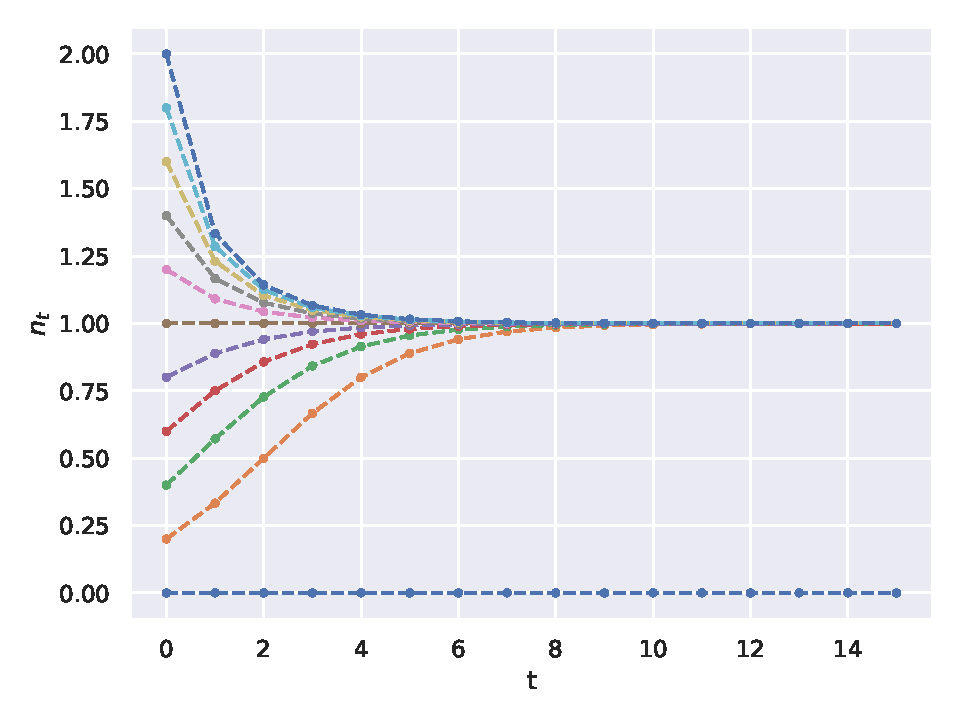
\includegraphics[width=\textwidth, height=0.8\textwidth]{Mapeo_r=2.pdf}
        \caption{}
        \label{01_Simulacion}
    \end{subfigure}
    \hfill
    \begin{subfigure}[b]{0.49\textwidth}
        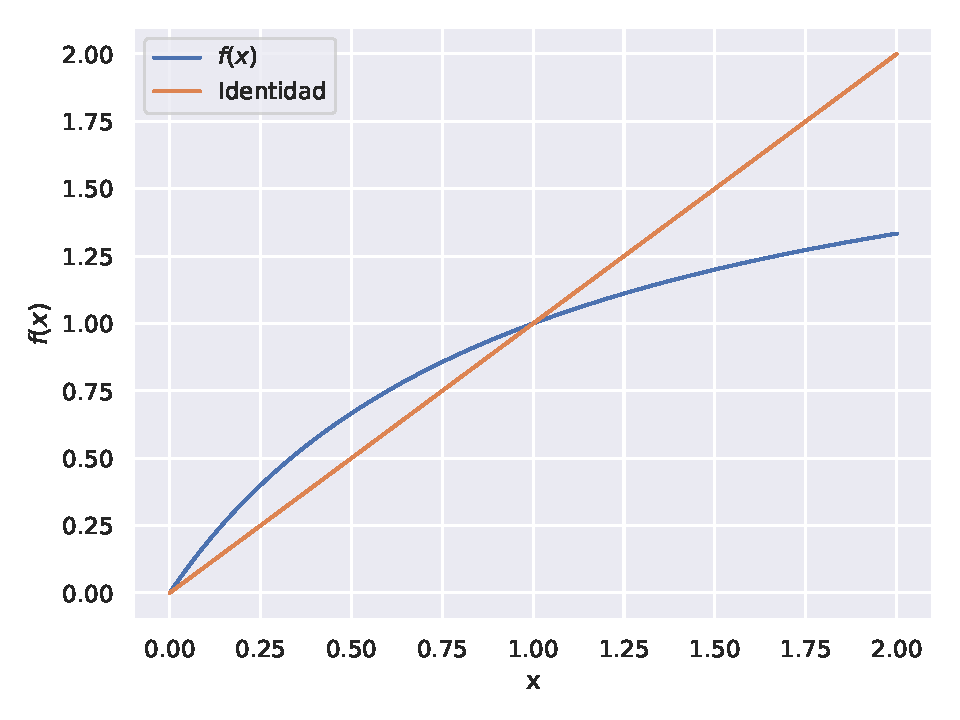
\includegraphics[width=\textwidth, height=0.8\textwidth]{Coweb_r=2.pdf}
        \caption{}
        \label{01_Coweb}
    \end{subfigure}
    \caption{Ene  la Figura (a) se observa la evolución del sistema para distintas condiciones iniciales para $r=2$ y $K=1$, mientras que en la Figura (b) se observa un gráfico \textit{Coweb} para los mismos parámetros.}
    \label{PONER_LABEL}
\end{figure}

\rojo{Falta mostrar que pasa para $r<1$. Acalrr lo del signo de K.}

En caso de que $r=1$, la Ec. \ref{eq:Mapeo_Beverton-Holt} se reduce a $n_{t+1} = n_t$, en donde todos los $n$ son puntos fijos, pero el comportamiento no es muy interesante.